%% nabbed from http://tex.stackexchange.com/questions/19982/how-do-i-add-parfor-in-algorithmic-environment
% declaration of the new block
\algblock{ParFor}{EndParFor}
% customising the new block
\algnewcommand\algorithmicparfor{\textbf{parfor}}
\algnewcommand\algorithmicpardo{\textbf{do}}
\algnewcommand\algorithmicendparfor{\textbf{end\ parfor}}
\algrenewtext{ParFor}[1]{\algorithmicparfor\ #1\ \algorithmicpardo}
\algrenewtext{EndParFor}{\algorithmicendparfor}


\section{DayMOPS}
\label{linking}

Sufficiently bright moving objects which are observed by the LSST
telescope will generate DiaSource detections, stored in the LSST
DiaSource detection catalog.  The LSST DiaSource detection catalog
will also hold detections from a variety of non-moving object sources,
including transient phenomena and artifacts of image processing.

The LSST DayMOPS system is responsible for finding previously unknown
moving objects within the LSST DiaSource catalog.  Due to the large
number of detections expected, and the sometimes-unpredictable
behavior of asteroids with unknown orbits, a structured and
carefully-designed system is necessary to perform this searching and
discovery in a computationally efficient manner.






\subsection{Orbits}
Heliocentric orbits describe an orbit around the Sun.  Generally,
asteroids, planets and other solar system objects follow elliptical
paths, with the Sun as their focal point.  These paths are described (in general
practice as well as the LSST Moving Objects catalog) with a Kepler
orbit, which describes an ellipse using six parameters. 

For purposes of DayMOPS and NightMOPS, we assume that a well-fitted
Kepler orbit should be sufficient to predict the location of an object
well into the future or past.  

To simplify the problem, we will not attempt to deal with objects
which do not follow conventional heliocentric orbits, such as
loosely-coupled binaries or planetary satellites.


\textbf{TBD: Illustration of a Kepler orbit - Wikipedia has a good one.}


\subsection{Orbit Determination and The Linking Problem}
Orbit determination refers to the problem of identifying an object's
orbit given a well-spaced set of detections of that object.  The
problem of orbit determination has been studied extensively \textbf{
  CITATIONS HERE }, and several software tools exist which can, given
a set of detections, identify an orbit which could have generated them
or identify that no such orbit could exist.We entrust that a suitable
outside tool will be chosen to handle this problem.

This leads to the non-trivial problem of correctly grouping sets of
detections by the unknown object which generated them, and reporting
these detections to an orbit determination tool.  This is the \textbf{
  linking problem}.  The majority of efforts in the DayMOPS system
have been directed at constraining the number of linkages which are
passed to the orbit determination tool, and at methods for discovering
those linkages quickly.

Fortunately, the well-known linear and quadratic approximations of asteroid
motion can be used both to predict possible linkages, and reject those
which are obviously untenable.  

\subsubsection{Linear and Quadratic Models}

\begin{figure}[ht]
  \centering
    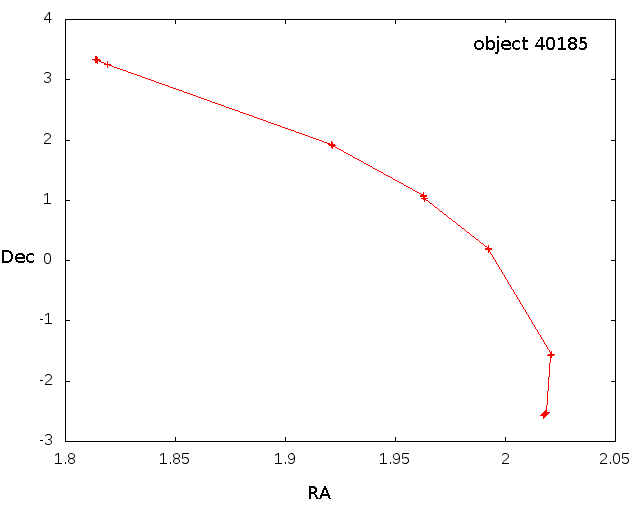
\includegraphics[width=10cm]{illustrations/4.png}
    \caption{ A plot of simulated observations of object 40185 on the
      sky.  Though the observations span only one week, a pronounced
      quadratic path is visible.  Note that the object is observed two
      or more times on each night.}
\label{objectPlotted}
\end{figure}



In order to discover and identify new objects, astronomers have
traditionally used sky-plane approximations to predict and model the
behavior of solar system objects for which a true orbit is not yet
known.  As a general rule of thumb, objects are said to move linearly
(with a more or less fixed velocity) in RA and Dec over the course of
a single night and quadratically (having velocity and some
acceleration) in RA and Dec over the course of a month.  These are, of
course, approximations, and linear and quadratic fits will inevitably
contain some error.  An example of one object with a clear quadratic
path over seven days is show in Figure~\ref{objectPlotted}.

Given many detections which may or may not be attributable to one or
more asteroids, these approximations are used to help determine which
detections could plausibly be linked.  If several detections over the
course of a single night do not follow a roughly linear path, we trust
that they could not have been attributable to the same object; if
several detections over the course of a month do not follow a roughly
quadratic path, we will trust that they could not be attributable to
the same object.  By ignoring the obviously implausible linkages, we
significantly reduce the number of hypothetical linkages we must
investigate.

Of course, since these are merely approximations, it is almost
inevitable that some correct linkages will be rejected.  In
particular, some near-Earth-objects (NEOs) may exhibit sky-plane
behaviour not consistent with these rules of thumb.


\subsubsection{Higher-order Sky-Plane Models}
\textbf{TBD: Tim's methods go here - the assumed topocentric distance, topocentric correction, higher-order fits}


\subsection{The Linking Pipeline}
The linking pipeline is responsible for finding sets of detections
which may be attributable to the same moving object and sending them
to the Orbit Determination stage, which will either accept them as a
true linkage with an associated orbit or reject them as incorrectly
linked.  

To deal with the scale and complexity of discovering plausible
multi-night linkages for unknown objects, the DayMOPS system is
designed as a pipeline of several stages, building increasingly
sophisticated linkages at each step until multi-night linkages
suitable for orbit determination are discovered.  Specifically, we
move from individual detections to nightly, linear \textbf{tracklets},
to eventual multi-night, quadratic \textbf{tracks} suitable for orbit
determination.  These tracks are filtered using a slightly more
sophisticated (but simpler than full orbit-space) model of asteroid
motion, to more quickly reject the (often numerous) mislinked tracks.


\begin{figure}[ht]
  \centering
    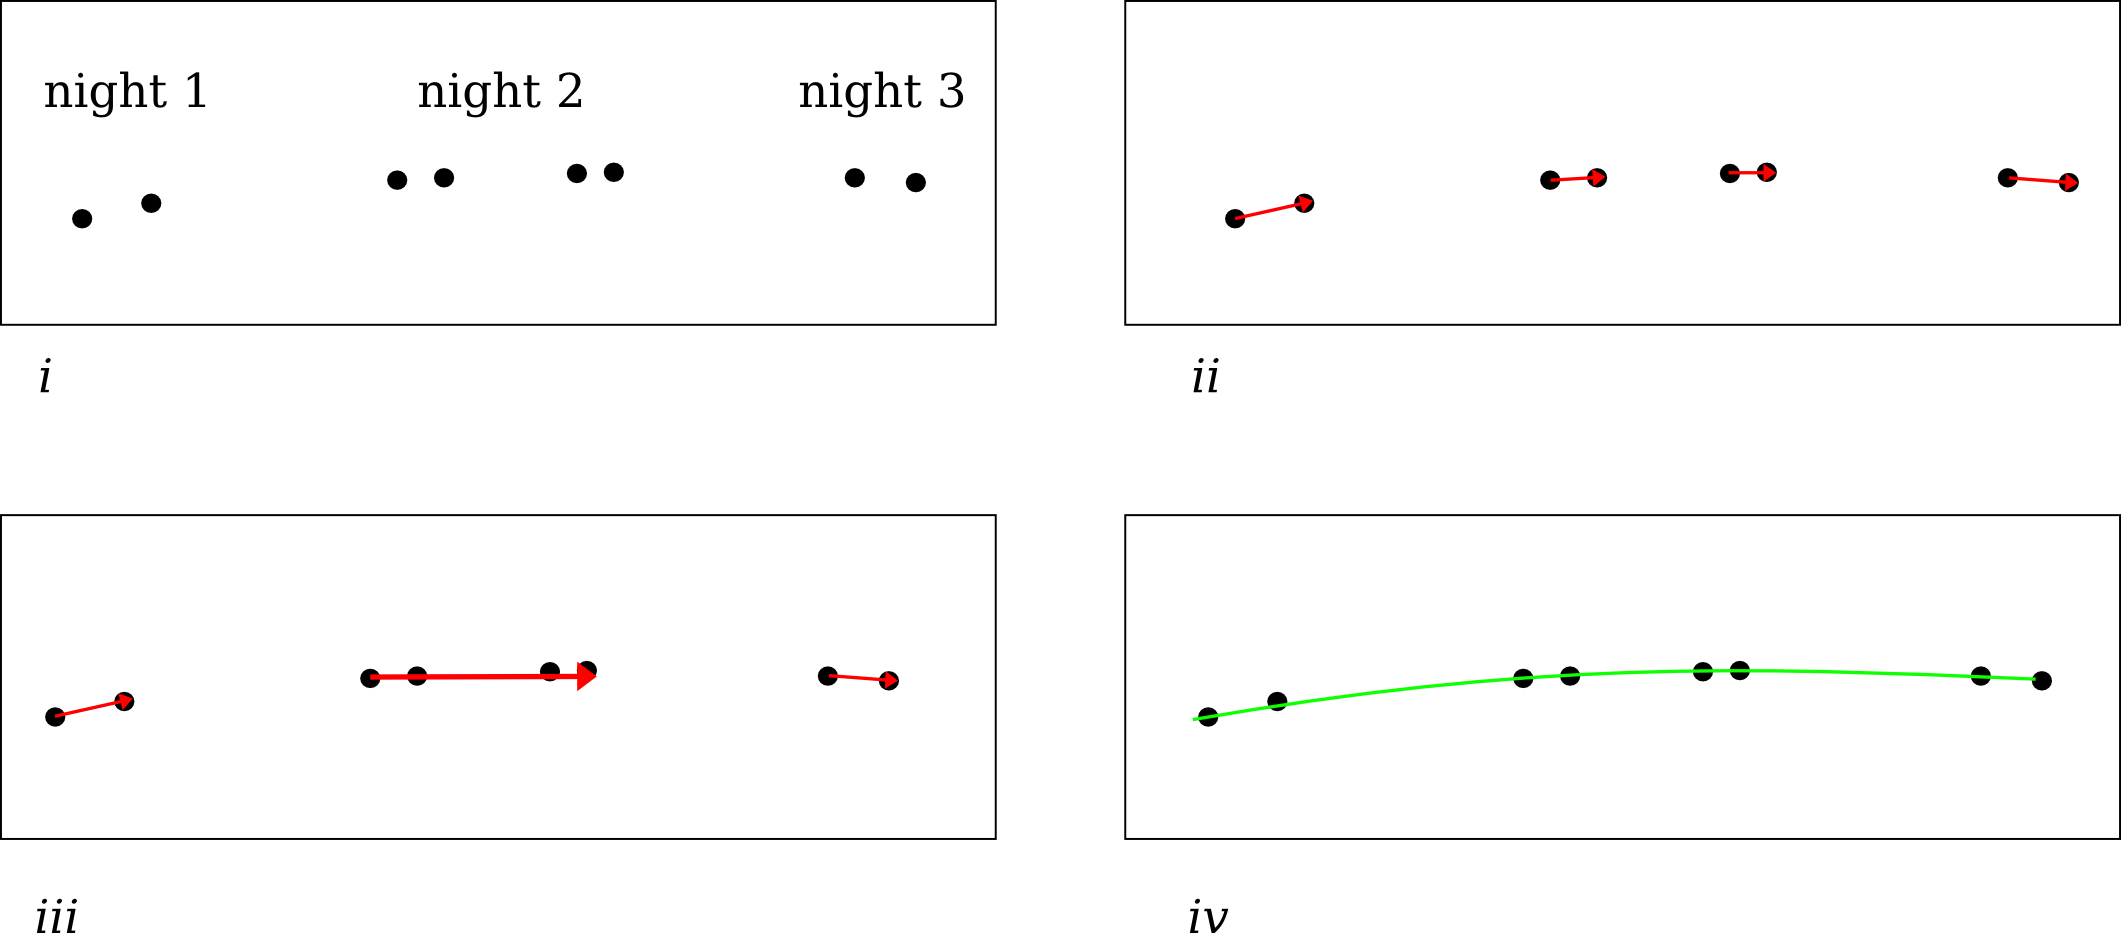
\includegraphics[width=16cm]{illustrations/oneObjectMops.png}
    \caption{ An illustration of how DayMOPS linkage might be applied
      to a single object.  In $i$, the object is observed on three
      nights; on the first and last night, it gets two detections per
      night, but on the second night it gets four.  In $ii$, initial
      tracklets are generated; time separation of visits on the second
      night is such that we get two tracklets.  In $iii$, we merge the
      tracklets from the second night so there are only three
      tracklets.  In $iv$, we attempt inter-nightly linking and
      generate a single track.}
\label{objectPlotted}
\end{figure}


Note that tracklets and tracks represent hypothetical linkages, many
of which may be incorrect.  A single detection may exist in several
tracklets and/or several tracks.  A given tracklet may be found in
multiple tracks.  Some detections may never be linked into any
tracklet; some tracklets will never be linked into any track.  

%The
%DayMOPS system is built using methods and algorithms intended to
%efficiently find plausible hypothetical linkages without wasting much
%computational time or storage on finding unlikely linkages.


%% TBD: Describing topocentric correction goes here?  It has to go
%% somewhere.  It is only performed on the data sent to linkTracklets,
%% but this isn't really central to understanding the vtrees algorithm
%% - though it does effect the data ``seen'' by linkTracklets
%% throughout.


\subsection{Building Tracklets}

\textbf{ possible illustration: show Dec/time for two images, then tracklets in Dec/time}

\textbf{Tracklets} are linkages between DiaSource detections occuring
within the same night. By creating tracklets, DayMOPS can find
sky-plane position and velocity estimates for sets of detections which
may belong to the same solar system objects.  The use of tracklets
also simplifies the downstream work of track generation, which
attempts to find sets of detections with a good
position/velocity/acceleration fit on the sky-plane; since tracklets
have known position and velocity, the track generation phase needs
only to find those tracklets compatible within some acceleration
factor.

Correctly-linked tracklets from a given object are needed to generate
a good track for that object and eventually discover its orbit.
However, if these useful tracklets are too deeply buried among very
large numbers of other tracklets, then the job of tracklet linking
will become extremely slow and expensive.  Generally, these other,
unwanted tracklets are false tracklets (mislinkages between detections
not attributable to the same object), though in special conditions
large numbers of correctly-linked but redundant tracklets can cause
pain as well (this will discussed in \ref{collapseTracklets}).

In order to ensure that tracklet-generating images are acquired, it is
necessary to ensure that fields of the sky are visited two or more
times within an accepted time period each night. To constrain the
number of tracklets, we impose a maximum apparent velocity on the
tracklets, and also require that sky fields be revisited within a
fairly short time period ($\leq 90$ minutes is the current rule).
Raising the maximum velocity threshold enables one to find
faster-moving objects, and raising the maximum allowed revisit time
also enables one to generate tracklets in more fields of the sky;
however, increasing either of these thresholds also increases the
search space and can significantly increase the number of mislinked
tracklets, greatly increasing the cost downstream.




\subsubsection{The findTracklets Software}

The process of initial tracklet creation is accomplished by the
findTracklets software.  Later refinement of tracklets is accomplished
by collapseTracklets and additional filters.

\subsubsubsection{Algorithm} 

The findTracklets software is responsible for finding pairs of
detections which occur within a fixed time threshold, and have
apparent velocity below a given threshold.  For a given detection and
a set of image times, one can calculate the maximum distance an object
could have travelled at each time using the velocity limit.  To find
detections with which the query detection could be linked, one can
imagine searching a circular region in the later images based on this
distance.

\begin{figure}[ht]
  \centering
    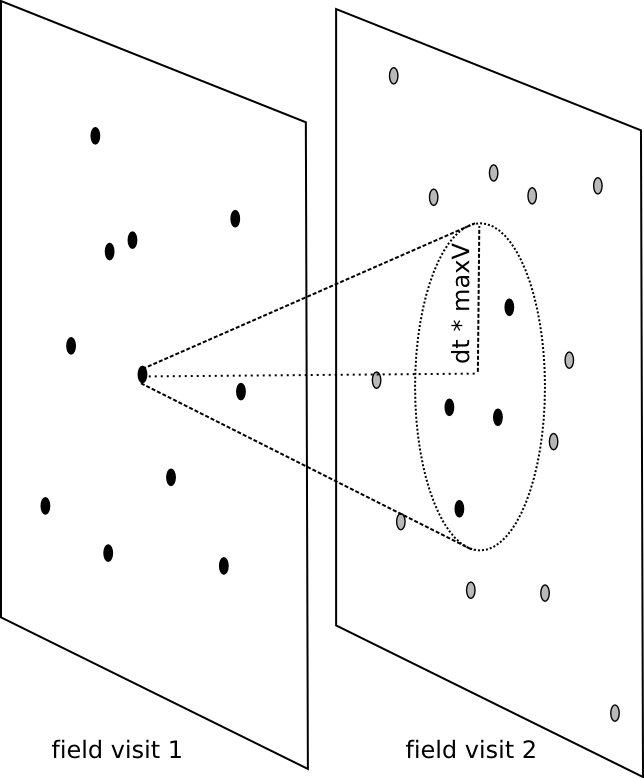
\includegraphics[width=6cm]{illustrations/findTracklets-onequery.png}
    \caption{ An example of searching for compatible second endpoints
      for a given detection.  The first detection and each of the
      second endpoints will be used to create a new tracklet.}
\label{findTrackletsIllustrated}
\end{figure}


Fortunately, this can be
accomplished in a fairly straightforward way through the use of
KD-Trees.  KD-Trees are a data structure which allows for quickly and
efficiently performing range searches on points in space
\citep{bentley_kdtrees}.  A KD-Tree-based method for building
tracklets was first contributed by Jeremy Kubica for his PhD thesis
\citep{kubica_thesis}.  For findTracklets, 2-Dimensional KD-Trees are
used, covering the space of (RA, Dec).  Given a detection and trees
containing detections from later images, we can use range searches to
quickly find nearby detections in those later images and use them for
the creation of tracklets.

\begin{figure}[ht]
\begin{algorithmic}[5]
\Require $I$ is a set of images, each of which has an associated exposure time and contains a set of detections
\State \Comment{Create a 2D KD-Tree for each image, holding detections from that image.}
\State $T \gets \emptyset$
\For {$i \in I$}
  \State $t \gets$ Make2DTree$(i.detections)$
  \State $t.time \gets i.time$
  \State $T \gets T \cup \{t\}$
\EndFor
\State \Comment{Use these trees to discover the actual tracklets.}
\State $tracklets \gets \emptyset$
\For {$t_1 \in T$}
  \State $later \gets \{t_i \in T : 0 < t_i.time - t_1.time < maxDt\}$
  \For{$d \in t_1.detections$}
     \For{$t_q \in later$}
 
       \State \Comment{Use time between images and max velocity to
         calculate the max travel distance}

        \State $dt \gets t_q.time - t_1.time$
        \State $dd \gets dt * maxV$
        \State \Comment{Use KD-Tree range search to find detections within max travel distance}
        \State $tracklets \gets tracklets \cup t_q.$rangeSearch($d.ra, d.dec, dd$)
     \EndFor
   \EndFor
\EndFor
\Return{$tracklets$}
\end{algorithmic}

\caption{Pseudo-code for the findTracklets algorithm.  2D (RA, Dec)
  trees are created for each image; for each detection, later trees
  are searched for nearby detections. }
 \label{findTrackletsAlgorithm}
\end{figure}


Note that because the sky is a sphere, notions of ``distance'' and
``velocity'' can become slightly confusing, especially near the poles.
Fortunately, both the KD-Tree library used and the findTracklets
software are sufficiently clever to use actual great-circle distance
and velocity for their queries, so that tracklets near the poles are
not missed.  The software should also be impervious to wrap-around
errors - objects which move between, say, $359.9 \degree$ in RA and
$.01 \degree$ in RA will be detected.  The Appendix \ref{kdTreeLib}
explains the KD-Tree library used in greater detail.  







%%%%%%%%%%%%%%%%%%%%%%%%%%%%%%%%%%%%%%%%%%%%%%%%%%%%%%%%%%%%%%%%%%5
%% COLLAPSE TRACKLETS
%%%%%%%%%%%%%%%%%%%%%%%%%%%%%%%%%%%%%%%%%%%%%%%%%%%%%%%%%%%%%%%%%%5


\subsection{Improving and Filtering Tracklets} \label{collapseTracklets}
If a field of the sky gets multiple revisits, or more than two visits
within the time window, it is possible that findTracklets will find
more than one true tracklet associated with that object.  This can
generated needless downstream work, because the number of tracklets is
larger, and if the multiple true intra-nightly tracklets are never
linked together, then useful data (additional detections of the
object) can be lost, or may need to be pieced back together later.

In particular, in ``deep drilling'' operations, the telescope will
repeatedly image the same field of sky many times in a short period.
In these fields, the number of tracklets generated for an object will
grow like $O(n^2)$ where $n$ is the number of times the object is
seen, as each possible pair of detections will be linked.  This can
generate a huge number of tracklets, making later work exceptionally,
and needlessly, difficult.  Even in more conventional cadences, in
which an object gets two or more tracklets per night, combining those
tracklets can significantly decrease downstream workload.

The tracklet improvement and filtering stage attempts to remedy this
problem by joining together colinear 2-detection tracklets into
higher-cardinality (3 detections or more) tracklets.


\paragraph{Special Considerations}
There is a small risk that occasionally, a true 2-detection tracklet
be merged into a larger tracklet which is mislinked.  This is rare, as
it can only occur when a true tracklet is colinear with a mislinked
tracklet, but it is not strictly impossible.



\subsubsection{The collapseTracklets Software} 

The tracklet refinement and filtering stage actually consists of
several steps, which can be iterated as necessary.  The first and most
important stage is the collapseTracklets stage, which finds roughly
colinear tracklets and merges them.  

To accomplish this, a method similar to the Hough transform is used.
An intermediate time, $t_c$ is selected (we use the average time of
the first and last detections) and use the apparent linear motion of
the tracklets to project their location at $t_c$.  We then store these
projected (RA,Dec) locations and the angle/velocity of each tracklet.
At this point, colinear tracklets should have similar positions and
motion vectors, making them easy to find.  This is accomplished with a
series of range searches, which of course can be implemented with 4-D
(RA, Dec, angle, velocity) KD-Trees.  The full pseudo-code is
presented in Figure \ref{collapseTrackletsAlgorithm}.

\begin{figure}[ht]
\begin{algorithmic}[5]
  \Require $T$ is a set of intra-nightly tracklets, $D$ is the set of nightly detections from which $T$ was created, $range$ is a 4-tuple of tolerances for RA, Dec, angle and velocity.
  \State $t_c \gets midpoint(\{ d_{time} : d \in D \})$
  \For {$t \in T$}
    \State Calculate $t$'s predicted location at time $t_c$, its motion angle and velocity
  \EndFor
  \State \Comment{Create a 4D KD-Tree of the tracklets on their projected RA, Dec position and motion angle/velocity.}
  \State $tree \gets$ Make4DTree$(T)$
  \State $outTracklets = \emptyset$
  \For {$t \in T,\ t$ has not already merged with another tracklet}
    \State \Comment{Find tracklets with projected location, motion similar to that of $t$}
    \State $candidates \gets tree.$rangeSearch$(t_{projected\ position}, t_{angle}, t_{velocity}, range)$
    \For {$c \in candidates$} 
      \If{$c$ and $t$ do not contain different detections from the same image}
        \State $t.detections \gets t.detections \cup c.detections$
        \State mark $c$ as already merged
      \EndIf
    \EndFor
    \State mark $t$ as already merged
    \State $outTracklets \gets outTracklets \cup t$
  \EndFor
  \Return{$outTracklets$}
\end{algorithmic}

\caption{Pseudo-code for the collapseTracklets algorithm. A 4-D KD-Tree over RA, Dec, angle, velocity is constructed using the projected locations and motion of the tracklets.  Tracklets which are similar in this 4-D space are roughly colinear, so they are merged and written to output}

\label{collapseTrackletsAlgorithm}

\end{figure}

Currently, collapseTracklets handles wrap-around, but otherwise treats
the sky as a flat (RA, Dec) plane when calculating the projected
positions of tracklets.  This is acceptable for tracklets close to the
ecliptic, but not sufficient closer to the poles.  This should be
fixed when possible.

Because the collapseTracklets algorithm does linking in
parameter-space, it is sometimes possible that the resulting tracklets
contain detections which are not quite colinear.  Also, some tracklets
may contain a superset of the detections present in other tracklets.
To address these, additional filtering stages are present.

\paragraph{Code and Usage}
The collapseTracklets algorithm is implemented in {\tt
  collapseTracklets.h} and {\tt collapseTracklets.cc}.  A command-line
interface is implemented in {\tt collapseTrackletsMain.cc}.  Run {\tt
  collapseTracklets -h} for usage hints.

Choosing an appropriate set of thresholds for collapseTracklets may be
difficult; with variable time between images, the amount of error on
velocity may differ from tracklet to tracklet.  Other factors come
into play as well; higher thresholds will lead to more correct
linkages as well as more incorrect linkages - which, as described in
the following section, can be ``undone'' later by purifyTracklets.  We
arrived at our current thresholds through simple trial and error.

\subsubsection{Tracklet Filtering Software}
The collapseTracklets algorithm attempts linking in parameter-space;
as a result, it is possible that tracklets which are not entirely
colinear may be merged.  This can be rectified using the
purifyTracklets algorithm, which removes detections from tracklets if
they are sufficiently off the best-fit line.  

Further, it is sometimes possible that a tracklet may link together a
set of detections already present in another, higher-cardinality
tracklet.  These ``subset tracklets'' are almost universally
unhelpful, and the removeSubsets algorithm may be used to efficiently
find and remove them from the active set of tracklets.


\begin{figure}[ht!]
\begin{algorithmic}[5]
  \Require $T$ is a set of tracklets, $rmsMax$ is a maximum root-mean
  squared residual on the tracklet's best-fit function to its
  detections

  \For {$t \in T$}
    \State $rms = RMS(t)$
    \While {$rms > maxRms, |t| > 2$} 
      \State remove the worst-fitting detection from $t$
      \State $rms = RMS(t)$
    \EndWhile
  \EndFor
  \Return{$outTracklets$}
\end{algorithmic}

\caption{In purifyTracklets, poorly-fitted detections are ``pruned''
  from tracklets. In certain degenerate cases, we may prune tracklets
  down to only two detections, in which case the two-detection
  tracklet is kept.}

\label{purifyTrackletsAlgorithm}

\end{figure}


The subset removal algorithm can be used for tracklets as well as
tracks.  It is presented in section~\ref{subsetRemoval}.








%%%%%%%%%%%%%%%%%%%%%%%%%%%%%%%%%%%%%%%%%%%%%%%%%%%%%%%%%%%%%%%%%%%%%
%%          LINKTRACKLETS
%%%%%%%%%%%%%%%%%%%%%%%%%%%%%%%%%%%%%%%%%%%%%%%%%%%%%%%%%%%%%%%%%%%%%


\subsection{Building Tracks}

With tracklets already assembled, we should have many linkages
representing the position, location, and velocity of the various
objects observed, as well as ``false'', mislinked tracklets.  While
tracklets have only linear motion, tracks have quadratic paths; in the
track building phase, this is always calculated as a pair of quadratic
functions in RA and Dec, rather than a single motion vector.  By
making use of this quadratic approximation of motion, valid for
approximately one month, we can move a sliding window of about 30 days
over the data, looking for tracklets which could be linked by some
quadratic acceleration factor.  As we find these linkages, we will
also apply some additional filters to avoid reporting those which are
considered too implausible (this will be described in
\ref{trackFilters}).

Generally, the track generation phase is the most computationally
expensive task in DayMOPS processing; note that unlike other stages,
which consider only a night's-worth of data at a time, it must
consider tracklets from many nights and find linkages between them.
This task becomes far more difficult if the number of tracklets is
very large, either because the source data was very dense or the
thresholds were set very high, or because of poor refinement/merging
of intra-nightly tracklets.  Further, the relative looseness of the
quadratic approximation and the relative scarcity of data can make
track generation yet more difficult, as many plausible tracks may be
discovered.

Fortunately, a very clever algorithm for performing this track
discovery was presented by Kubica et al. (\citet{kubica_thesis},
\citet{Kubica:2005:MTA:1081870.1081889}).  In essence, the idea behind
the algorithm is to build per-image 4D-Trees of (RA position, Dec
position, RA velocity, Dec velocity), and use these to hold the
tracklets, indexed by position/velocity.  We then imagine the KD-Trees
as hierarchical bounding boxes, and consider pairs of bounding boxes
from different nights, calculating whether they could be linked by
some acceleration factor less than our maximum acceleration threshold.
If the boxes could be linked, then a track may exist within their
contents and we continue searching bounding boxes lower in the tree
hierarchy; if not, we know that no track of interest to us could pass
through the boxes and we can abandon searching immediately.  By using
the hierarchical structure of the KD-Trees, we can avoid searching in
large areas of tracklet-space where no track could ever exist, greatly
reducing our workload.


\subsubsection{Search Pruning}
\label{searchPruning}
In the linkTracklets algorithm, all tracklets starting in a given
image are placed in a single 4D-Tree over (RA position, Dec position,
RA velocity, Dec velocity)-space.  One tree is created for each of the
images.

Each KD-Tree node can be thought of as representing a bounding box in (RA
position, Dec position, RA velocity, Dec velocity) space.  Thus, it is
possible to calculate the acceleration needed for an object in one
bounding box in one tree to reach the second bounding box in a later
tree.  Because we are generally interested in tracks which have
acceleration within a fixed range (e.g. between $>.02 deg/day^2$ and
$<-.02 deg/day^2$), we can abandon searching at a given pair of
bounding boxes if the necessary acceleration is outside our range of
interest.

The minimum and maximum acceleration connecting two bounding boxes is
currently calculated as follows:


\begin{equation}
maxAcc = \min  \left(\begin{array}{ccc} & \displaystyle \frac{Node2.maxV - Node1.minV}{dt} \\
& \displaystyle \frac{2}{dt^2} \bigg(Node2.maxP_0 - Node1.minP_0 - Node1.minV \times dt \bigg) \\
& \displaystyle \frac{2}{dt^2} \bigg(Node1.maxP_0 - Node2.minP_0 + Node2.maxV \times dt \bigg) \end{array}\right)
% & \displaystyle parentMaxAcc, \\ jeremy says this shouldn't happen, even though it's in the code
\label{maxAcc}
\end{equation}

\begin{equation}
minAcc  = \max  \left(\begin{array}{ccc} & \displaystyle \frac{Node2.minV - Node1.maxV}{dt},\\
& \displaystyle \frac{2}{dt^2} \bigg( Node2.minP_0 - Node1.maxP_0 - \displaystyle Node1.maxV \times dt\bigg), \\
& \displaystyle \frac{2}{dt^2} \bigg(Node1.minP_0 - Node2.maxP_0 + Node2.minV \times dt\bigg) \end{array} \right)
%   & parentMinAcc, jeremy says this shouldn't happen, even though its in the code.
\label{minAcc}
\end{equation}


Note that this approach simplifies the problem by treating the sky as
a flat plane, which will be problematic near the poles.  However, the
above calculation appears to be the ``hot spot'' of the linkTracklets
algorithm and accounts for most of the computation time, and so
simplifying to reduce floating point costs greatly improves
performance.

In the code, this calculation is performed by the function 
{\tt updateAccBoundsReturnValidity} in {\tt linkTracklets.cc}.

\subsubsection{Recursive Tree-walk Using Pruning}

The linkTracklets algorithm makes use of pruning to quickly avoid
searching in areas where no track of interest could exist.  This can
be accomplished with a recursive walk over two KD-Trees representing
tracklets from different images.  As a simplified introduction to the
full algorithm, see Figure~\ref{simplifiedLinkTracklets} for a
two-tracklet-linking, ``endpoint-only'' version of the algorithm which
finds pairs of compatible tracklets on different nights.

\begin{figure}[ht!]
\begin{algorithmic}[5]
  \Require{$nodeA$ and $nodeB$ are KD-Tree nodes which hold tracklets
    from two different images on different nights, $minAcc$ and $maxAcc$
    specify the limits of accelerations which the user finds
    interesting.}
  
  \State $accRange = $ min/max acceleration to move from $nodeA$ to $nodeB$
  \If{$accRange$ does not overlap $(minAcc, maxAcc)$}
  \Return $\emptyset$
  \Else
  \If{$nodeA$ and $nodeB$ are leaf nodes}
  
  \State \Comment{When we hit a pair of terminal nodes, and their
    acceleration bounds are interesting, then we have found a set
      of tracklets which may be sufficient to create a track.}
    
    \Return $\{$tryToBuildATrack($nodeA$.tracklet, $nodeB$.tracklet)$\}$
    \Else
    
    \State \Comment{In order to ensure that this function sees
      nodes which are roughly the same size, we choose the larger
      node and ``split'' that one, recursing on its children.}


    \State $largerNode, smallerNode \gets orderBySize(nodeA, nodeB)$
    \State $leftRes \gets recurse(largerNode.\text{leftChild}, smallerNode, S)$
    \State $rightRes \gets recurse(largerNode.\text{rightChild}, smallerNode, S)$
    \Return $ leftRes \cup rightRes $
    \EndIf
    \EndIf
    
  \end{algorithmic}
  \caption{An endpoint-matching, two-tracklet version of the
    linkTracklets algorithm.  Note that if two nodes have no chance at
    holding a compatible tracklet (first ``if'' check) then their
    children are never searched; only if they may hold an interesting
    track are the children searched.  In this way, the algorithm
    avoids even examining a great number of KD-Tree node pairs and
    thus the pairs tracklets contained therein.}
  
  \label{simplifiedLinkTracklets}
\end{figure}

\paragraph{Support Tracklets, Support Nodes, and the Full LinkTracklets Algorithm}

For Orbit Determination, we require detections on at least three
nights.  The endpoint-only algorithm in \ref{simplifiedLinkTracklets}
will only attempt to find pairs of tracklets, giving tracks with only
two nights of observational data.  In practice, we seek to find tracks
with tracklets from three unique nights.  This could be accomplished
using various extensions to the endpoint-only algorithm, but it is
argued in \citet{kubica_thesis} and
\citet{Kubica:2005:MTA:1081870.1081889} that by far the most efficient
of these variants is called the algorithm called the {\bf vtrees} (for
``variable trees'') algorithm.

In the vtrees algorithm, we search for tracks with one or more
intermediate ``support'' tracklets in between the ``endpoint'' or
``model'' tracklets (the first and last tracklet).  To accomplish
this, the vtrees algorithm searches for compatible endpoint nodes as
in Figure~\ref{simplifiedLinkTracklets} but, as search progresses, maintains
a list of compatible ``support'' nodes - nodes which could hold useful
intermediate tracklets between the tracklets in the endpoint nodes.
These are filtered at each step, again using the equations
\ref{maxAcc} and \ref{minAcc}.  As the search descends through the
possible valid combinations of endpoint nodes, the support list is
filtered and refined.  When search terminates at a pair of leaf nodes,
the support nodes are used to find possible support tracklets.  If the
support list ever becomes empty, we can prune the searching at this
point, since we know no useful track could exist between the endpoint
nodes.

The full vtrees algorithm is presented in
Figure~\ref{linkTrackletsAlgorithm}.  This is the actual algorithm
implemented by the function {\tt doLinkingRecurse} from {\tt linkTracklets.cc}


\begin{figure}[ht!]
\begin{algorithmic}[5]

\Require{$nodeA$ and $nodeB$ are KD-Tree nodes which hold tracklets
  from two different images on different nights, $S$ holds a series of
  nodes from images take on nights in between $nodeA.time$ and
  $nodeB.time$, $minAcc$ and $maxAcc$ specify the limits of
  accelerations which the user finds interesting.}

\State $accRange = $ min/max acceleration to move from $nodeA$ to $nodeB$
\If{$accRange$ does not overlap $(minAcc, maxAcc)$}
    \Return $\emptyset$
  \Else
  
  \For{$supportNode \in S$}
  \If{$supportNode$ represents an awkwardly large portion of tracklet-space relative to $nodeA$ and $nodeB$}
    \State replace $supportNode$ with $supportNode.rightChild$ and $supportNode.leftChild$, coming back to them later
    \Else
    \If{no track with acceleration within $accRange$ could pass from $nodeA$ through $supportNode$ and into $nodeB$}
      \State remove $supportNode$ from $S$
    \EndIf
  \EndIf

  \If{$S$ is empty}
    \Return $\emptyset$ \Comment{There is no way to build a three-tracklet track using the contents of these nodes, so abandon searching.}
  \EndIf

  \EndFor
    \If{$nodeA$ and $nodeB$ are leaf nodes}

    \State \Comment{Again, try to build a track, this time using $S$ for intermediate tracklets}

       \Return $\{$tryToBuildATrack($nodeA$.tracklet, $nodeB$.tracklet, $S$)$\}$
    \Else

       \State $largerNode, smallerNode \gets orderBySize(nodeA, nodeB)$
       \State $leftRes \gets recurse(largerNode.\text{leftChild}, smallerNode, S)$
       \State $rightRes \gets recurse(largerNode.\text{rightChild}, smallerNode, S)$
       \Return $ leftRes \cup rightRes $
  \EndIf
\EndIf

\end{algorithmic}
\caption{The full vtrees algorithm, the actual algorithm implemented
  in linkTracklets.  At each recursion, $S$, the set of support nodes,
  is split based on the position, velocity, and acceleration range
  implied by the $nodeA$ and $nodeB$, the two endpoint nodes.  Note
  that if support nodes are periodically ``split'' and replaced with
  their chidlren if they too large relative to $nodeA$ and $nodeB$.}
 \label{linkTrackletsAlgorithm}
\end{figure}

In the algorithm, support nodes are filtered and possibly split (and
their children filtered) at each recursive step.  Choosing when to
split the support nodes is an important performance question.  If we
split too aggressively, then we will add more items to $S$ and be
required to filter a larger number of nodes at each recursion, which
will increase cost at each step.  If we split support nodes too
rarely, then the support nodes may become very large relative to the
endpoint nodes and we will often find that we have some compatible
support node, and thus continue searching - even in cases where, had
we split the support nodes, we would have seen that none of the leaf
nodes held by the larger box were consistent with our
position/velocity/acceleration range.  This leads to needless
searching when we should have simply terminated.

Currently, the cutoff for splitting is based on the spatial size of
the support node relative to that of the two endpoint nodes.  First
a weighting factor, $\alpha$, is calculated:

\begin{equation}
\alpha = \frac{supportNode.time - nodeA.time}{supportNode.time - nodeB.time}
\end{equation}

We then split the node if, for \textit{any} of the spatial axes (RA position, Dec position, RA velocity, or Dec velocity):

\begin{equation}
\bigg(\frac{width(nodeA.axis)}{\alpha} + \alpha \x width(nodeB.axis)\bigg) < 4 \x width(supportNode.axis)
\end{equation}

Where $width$ is the spatial extent of the node.  This approach was
developed by Jeremy Kubica through empirical testing, and may or may
not be optimal for our data; however, in our experience, it seems to
be effective.

The splitting and filtering of the support trees is implemented by
{\tt splitSupportRecursively} in {\tt linkTracklets.cc}.  This
function uses several helper functions, including the same {\tt
  updateAccBoundsReturnValidity} function used to check the
compatibility of endpoint nodes.


\subsubsection{Terminal Processing - Actual Track Generation}

Once a pair of endpoint tracklets and one or more support tracklets
have been found via the vtrees algorithm, we may attempt to finally
build a track from them.  This is relatively straightforward; three or
more tracklets with compatible acceleration, from three or more
nights, have already been found.  However, this acceleration factor is
rather approximate, as it is based on the position and velocity
estimate of the tracklets, not the best-fit to the detections held in
the tracklet.  Thus, at this point we actually start examining the
detections themselves.

First, we attempt to fit a simple quadratic to the detections in the
endpoint tracklets.  We reject the track if the best-fit acceleration
is too high or too low.  Next, we use the best-fit quadratic to
predict the locations of the hypothetical object at the time of each
support detection, and find those detections within some
user-specified threshold of the predicted location.  In the event that
there are multiple possible support detections at one of these image
times, the best-fitting detection is chosen.  If an insufficient
number of valid detections are found, we reject and do not build a
track.

If the nascent track has survived these initial filters, we pass it
onward to the more precise higher-order chi-squared-probability filter
described in \ref{trackFilters}.  If the track passes this final
filter, then at last it is added to our output set.


\subsubsection{Subtle Quirks}

\paragraph{Topocentric Correction}
As will be described in \ref{trackFilters}, we can generate more
precise fits and do more aggressive filtering if we first apply a
topocentric correction to the detections, converting from topocentric
coordinates to geocentric coordinates based on an assumed topocentric
distance.  For this reason, before the positions/velocities of the
tracklets are calculated, the trees are built or the linking algorithm
is run, topocentric correction is applied to the detections.  This
will have some (usually small) impact on all aspects of the search,
but will mostly be noticeable when filtering tracks.  



\paragraph{Spherical Geometry Issues}
Currently, the tracklet tree constructor in {\tt TrackletTree.cc} will
alter RA (and if needed, Dec) values so that all RA (and possibly)
values are stored on a contiguous 180-degree region.  This simplifies
the critical ``hot-spot'' calculations in {\tt
  updateAccBoundsReturnValidity}, since we do not need to check for
values which cross over the 0/360 line in RA.  However, this means
that if the input data covers too large an area of the sky then the
acceleration range calculation will likely fail, and thus the whole
algorithm will misbehave.

Further, As mentioned in section \ref{searchPruning}, we simplify the
math throughout track generation by treating the sky as a flat plane,
which will lead to significant distortion near the poles.  This
problem is often addressed by rotating the data in question so that it
is centered on the RA, Dec origin (0,0), where polar distortions are
minimal.  This could be done for the entire input set of detections,
but if the detections cover a sufficiently large area of the sky then
we will not significantly reduce the problem.  Temporarily
re-centering the relevant points at each call to {\tt
  updateAccBoundsReturnValidity} would likely work, but would probably
be quite expensive.  This is a problem which needs to be addressed
eventually, perhaps by changing the equations used in
\ref{searchPruning}, or per by rotating the bounding boxes per-query,
so that the endpoint images will always be roughly centered over the
origin.


\paragraph{Special Considerations of KD-Tree Construction} 

Astrometric error on detections will affect both the position and
velocities of true tracklets.  As a result, bounding boxes must be
extended to encompass not just the tracklets which they hold, but the
surrounding error bars.  Each tracklet will have a unique error bar on
its velocity, as tracklets will span different distances in RA and Dec
($dp$) and may also span different numbers of images and thus have
different $dt$:

\begin{eqnarray}
minV = (dp - 2\times astrom\_err)/dt  \\
maxV = (dp + 2\times astrom\_err /dt
\end{eqnarray}

Thus, each node in the tracklet KD-Tree will have its position range extended by:

\begin{eqnarray}
minP_0 = P_0 - astrom\_err \\
maxP_0 = P_0 + astrom\_err  
\end{eqnarray}
\\ and its velocity range will be extended to encompass the $minV$ and
$maxV$ of all its child tracklets.  These rules apply to leaf nodes as
well as non-leaf nodes, which must have bounds at least as great as
their child nodes.  Note that as a result of expanding the boxes
around tracklets, KD-Tree nodes may actually overlap.

Note that for linkTracklets, a leaf node's bounds should only extend
as far as the error bars around their tracklets, and the leaf non-leaf
nodes should encompass only the area around their children's bounds.
One of our early implementations did not follow this rule, and instead
partitioned the space in a ``top-down'' fashion as in the left side of
Figure~\ref{trackletTree}, and it then handled the issue of error bars
in the acceleration calculation function.  This was technically
correct, but lead to horrific performance - 1,000 or 10,000 times
slower than the current version, illustrated on the right side of
Figure~\ref{trackletTree}.  This is because the earlier version had
nodes which encompassed larger areas of tracklet-space and thus sets
of nodes were more likely to appear compatible, which results in less
search pruning.

\begin{figure}[ht!]
\centering
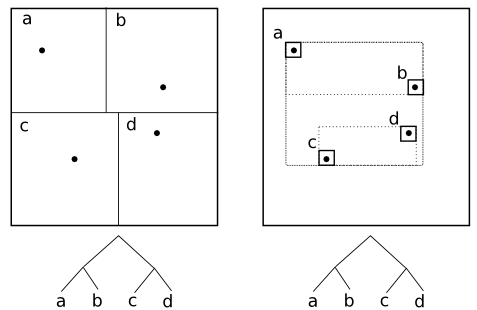
\includegraphics[width=10cm]{illustrations/kdTree_trackletTree.png}
\caption{Two possible ways of constructing a KD-Tree over four points.}
\label{trackletTree}
\end{figure}

The former type of tree is simpler to construct (and perhaps easier to
visualize when debugging).  This is the type of tree used in most the
other algorithms, which perform range searches and thus can extend
handle their error bars per-query by extending their ranges as needed.
However, the latter type of tree is the one needed for linkTracklets,
and is implemented by the KD-Tree subclass {\tt TrackletTree} in {\tt
  TrackletTree.cc}.


\paragraph{Performance Enhancements for Acceleration Range Calculation}
As noted earlier, the function {\tt updateAccBoundsReturnValidity},
which implements the equations \ref{maxAcc} and \ref{minAcc},
accounts for most of the CPU time spent in linkTracklets.  Thus,
optimizing performance in this section of code is critical.

Rather than evaluate all arguments to $\min$ and $\max$ functions at
the outset, the code attempts to evaluate each possible argument. If
it becomes clear at any point that inevitably $minAcc > maxAcc$, then
we know that the search can be pruned and the function returns
immediately.

As an additional optimization, we start with $minAcc$ and $maxAcc$ set
to the values used by our caller in the recursive searching. We know
that the caller was examining two endpoint nodes which were either
equal to or a parent of our current nodes, and thus our parents
$(minAcc, maxAcc)$ range will be greater than the one we
calculate. (For the initial start of the recursion, we use the
user-specified min/max acceleration thresholds, because we do not care
about any values outside this range anyway.)  By doing this, we
actually have a $maxAcc$ value available as soon as we calculate our
first possible $minAcc$ value and vice-versa; this allows the earliest
possible termination.  However, it does make the code somewhat more
confusing to read.

This confusion is somewhat amplified by the fact that this same {\tt
  updateAccBoundsReturnValidity} function is used for filtering
support nodes.  In this case, the initial $minAcc$ and $maxAcc$ values
are taken from the acceleration range calculated when examining the
endpoint nodes $nodeA$ and $nodeB$, since we are not interested in
finding acceleration values which connect $nodeA$ and a support node
unless they also connect the support node to $nodeB$.








%%%%%%%%%%%%%%%%%%%%%%%%%%%%%%%%%%%%%%%%%%%%%%%%%%%%%%%%%%%%%%%%%%%%%%%%
%%      TRACK FILTERING
%%%%%%%%%%%%%%%%%%%%%%%%%%%%%%%%%%%%%%%%%%%%%%%%%%%%%%%%%%%%%%%%%%%%%%%%
\subsection{Filtering of Tracks}
\subsubsection{Higher-Order Fits and Chi-Squared Probability Filtering}
\label{trackFilters}
Some more information on implementation of Tim's fitting and
chi-squared filter and the software. Stats on ground-truth fitting,
possible needs for improvements.

\subsubsection{Subset Removal}
\label{subsetRemoval}
Some tracks are {\bf subset tracks} of other tracks; that is,
occasionally detections linked by one track found by linkTracklets
will be a subset of those linked by another track in the same output
set.  This can arise for a variety of reasons, but occurs most
commonly when a real object generates tracklets on four or more nights
within a linking period. We generally expect that these subset tracks
are unhelpful, and because they increase the size of the set of tracks
sent to orbit determination, they are possibly costly.

Finding and removing subset tracks could be accomplished with a very
naive double-for loop over the set of tracks, but of course this does
not scale to larger data sets ($O(n^2)$ for $n$ tracks).  A more
efficient algorithm uses a detection-to-track ``reverse-map'' $R$,
which maps from each detection to the set of tracks holding that
detection.  This is easy to construct for a set of tracks $T$:

\begin{algorithmic}[5]
  \For{$t_i \in T$}
  \State $R[d_j] = \{\}$
  \EndFor
  \For{$d_j \in t_i$}
  \State $R[d_j] = R[d_j] \cup t_i$
  \EndFor
\end{algorithmic}

We may then use the algorithm from
Figure~\ref{subsetRemovalAlgorithm}, which makes use of this
reverse-map.  The underlying idea is this: for each track $t_i$, we
seek to find any track containing all the detections in $t_i$; any
track containing all these detections must be equal to or a superset
of $t_i$.

\begin{figure}[h!]
\begin{algorithmic}[5]
\For{$t_i \in T$}
  \State candidates = $T$
  \For{$d_j \in t_i$}
    \State candidates = candidates $\cap$ $R[d_j]$
  \EndFor
  \If{$|$candidates$| >$ 1}
    \State $t_i$ is a subset of some other $t_j \in T$; discard it
  \Else 
    \State keep $t_i$
  \EndIf
\EndFor
\end{algorithmic}
\caption{Psuedocode for the subset removal algorithm}

\label{subsetRemovalAlgorithm}
\end{figure}

Subset tracklets can also occur when collapseTracklets is used.  The
same algorithm and software can be used to remove subset tracklets
from a set of tracklets as well.

The reverse-map is implemented with a C++ {\tt std::map}, allowing
logarithmic-time lookups, and its contents are C++ {\tt std::set}s,
which allowing linear-time intersection calculations.  However, both
structures are implemented with trees; between the tracks themselves
and these tree structures, this algorithm can require significant
amounts of memory, and no distributed-memory equivalent is currently
known to us.  Fortunately, we have had good luck with distributed
shared-memory approaches for large data sets {\bf self-cite?}.



\subsection{Notes on Software Interfaces}

\subsubsection{Accomodations for Large Data Sets}
\label{largeData}
Over the course of our experiments, we discovered that under some
circumstances, tools may return some very large data sets - larger
than the memory available on our development machines.  Though RAM
sizes may grow over time, it is likely that DayMOPS users will
continue to experiment with increasingly dense noise or loose limits,
resulting in increasingly large numbers of tracklets or tracks.

To help deal with this problem, the {\tt  findTracklets} and
{\tt linkTracklets} functions can be configured to output their results
in various ways; they can be configured either to store their results
in memory and return them (much like a normal function call) or to
return nothing and write results directly to file.  If the user is
confident that the data set to be returned will fit in memory, the
former is more elegant, but for our experiments we always write to
file first, in case the number of tracklets or tracks discovered is
large.

The {\tt findTracklets} and {\tt linkTracklets} functions each take as
an argument an object of type {\tt findTrackletsConfig} or
{\tt linkTrackletsConfig}; each type has a public member variable
called {\tt outputMethod} which can be set.  {\tt findTracklets.h} and
{\tt linkTracklets.h} each contain enum types which can be used to set
these flags.

Dealing with larger-than-memory data sets as input to our software
tools is a more significant problem.  We generally assume that the
number of input detections will fit in memory, and that KD-Trees of
these detections will also fit in memory.  This has always been the
case, and fortunately it is easy to predict whether a set of
detections will fit in memory or not.  However, the number of
tracklets or tracks may, depending on the data and configuration of
the software, grow to be quite large, and is not trivially
predictable.  For software which uses tracklets or tracks as its input
data and operates on them in bulk (including {\tt collapseTracklets},
{\tt removeSubsets}, and {\tt linkTracklets}), this may be problematic.



\subsubsection{Parallelization}
\label{parallelization}

We have parallelized the various linking stages of DayMOPS using
multithreading, implemented using OpenMP.  This allows multiple CPU
cores to work simultaneously on the data set, but does not address the
problem of partitioning the data sets between machines.  This means
that multithreading can be effective in large-memory environments, but
does not attempt to solve the problem of larger-than-memory data sets.

The issue of larger-than-memory data sets could be addressed in
several ways: through (OS-level or implementation-level) distributed
shared memory, algorithmic changes, or simply requiring large-memory
machines.  We have had good luck using kernel-level distributed shared
memory provided by the vSMP software on the Gordon cluster at San
Diego Supercomputing Center.  This software runs inside the OS kernels
of various machines connected via network, and provides the appearance
that all CPUs and RAM on the various machines are shared on a single
motherboard.  A similar effect could be achieved through explicit use
of a user-level distributed shared memory library (such as memcached),
but would require additional coding.

\subsubsubsection{Parallel FindTracklets} In our current version, we
parallelize the work being done per-detection.  This is achieved with
a simple \textbf{parallel for} loop replacing the \textbf{for} loop at
line 12 in the pseudocode at Figure~\ref{findTrackletsAlgorithm}.  Because the amount of work
done will vary per-detection, depending on how many possible second
endpoints are found, we use dynamic thread scheduling as opposed to
static scheduling.  The only critical section used is the writing of
results, otherwise there is no need for inter-processor
synchronization or communication.

The tracklets reported by parallel findTracklets should be identical
to those reported by serial findTracklets, though the order in which
they are reported may differ.


\subsubsubsection{Parallel CollapseTracklets} The work done is
parallelized on a per-tracklet basis.  Again, this is achieved with a
simple \textbf{parallel for} loop replacing the \textbf{for} loop at
line 8 of Figure~\ref{collapseTrackletsAlgorithm}.  The writing of output is
inside a critical section, as in parallel findTracklets.

Unlike findTracklets, the work done in the parallel region of
collapseTracklets is not entirely independent; different threads may
read and write the ``already merged'' flags on tracklets.  This leads
to a potential consistency problem, with several possible solutions.
One approach would be to enforce strict locking on every read/write to
the ``already merged'' flags.  This has the disadvantage of
potentially scaling very badly, since the reads/writes are extremely
frequent and synchronization costs could be quite high.  It is also
problematic in that it creates potential for deadlocks if not
implemented very carefully.  A second approach would be to disregard
the flags entirely, which would be quite simple to implement. However,
in cases where objects may generate many tracklets (e.g. deep stacks,
which can see $n^2$ tracklets given $n$ observations) this would
result in a significant amount of redundant work being performed.  We
took a third approach, which attempts to compromise these two: we do
not enforce strict locking on the ``already merged'' flags, and simply
allow that there may be stale reads occasionally.  These stale reads
may lead to redundant work, but because we expect that they will be
uncommon, and hopefully should not have a big impact on performance.
The redundant work will lead to redundant tracklets in output, but we
expect them to be removed by the removeSubsets stage.

It is also important to note that because of the ``already merged''
flags, results from collapseTracklets are nondeterministic in a
multi-threaded environment.  Consider the unusual case in which
tracklets $t_a$ and $t_b$ are sufficiently close in the tree, and
$t_b$ and $t_c$ are sufficiently close in the tree, but $t_a$ and
$t_c$ are not sufficiently close in the tree, and querying for one
will not return the other.  Depending on which tracklet is first
visited and queried for similar tracklets, tracklet $t_b$ may be
merged with either $t_a$ or $t_c$, at which point it will be flagged
and never considered again.  As a result, output from parallel
collapseTracklets runs is expected to vary, and not just with regard
to ordering, albeit quite slightly.


\subsubsubsection{Parallel LinkTracklets} 

LinkTracklets looks for tracks which could start in a given image and
end in another given image.  Usually, the number of possible
start/endpoint image pairs is fairly large, so this provides a natural
axis of paralellism.  The psuedocode for the parallel linkTracklets is presented in Fig. \ref{parallelLinkTracklets}.


\begin{figure}[h!]

\begin{algorithmic}[5]

\Require{$T$ is a set of per-image tracklet trees}
\State $work \gets \emptyset$
\For{$t_i \in T$}
  \For{$t_j \in T$ and $t_j$ happens $\ge 2$ nights later than $t_i$}
    \If{there are sufficient support trees between $t_i$ and $t_j$}
    \State add $t_i, t_j$ to work
    \EndIf
  \EndFor
\EndFor

\ParFor{$w \in$ work}
  \State $t_i, t_j \gets w$
  \State $sup \gets $ trees from images between $t_i$ and $t_j$
  \State use vtrees algorithm (Fig. \ref{linkTrackletsAlgorithm}) to find tracks starting in $t_i$, ending in $t_j$ and passing through $sup$ 
\EndParFor

\end{algorithmic}
\caption{Psuedocode for parallel linkTracklets.  First, usable pairs of images are identified in a single thread, then the searching between these pairs of images is performed in parallel by multiple threads.}
\label{parallelLinkTracklets}
\end{figure}

The work done inside the parallel sections is naturally independent,
and so the only critical section is the writing of output.  The
parallel linkTracklets should return the same tracks discovered by the
sequential version, though the order of their discovery may differ.


\subsubsubsection{Parallel Subset Removal} 

Again, the subset removal algorithm contains an outer \textbf{for}
loop which provides an obvious axis of parallelism.  The \textbf{for}
loop at line 8 of Figure~\ref{subsetRemovalAlgorithm} is simply
changed to a parallel \textbf{for} loop to achieve multi-threading
parallelism.  

The work done in the parallel section is natrually independent, so the
only critical section is the writing of output.  The results of
parallel subset removal should be identical to that of the sequential
version, except for the ordering.





\subsubsubsection{Orbit Determination} 

Orbit Determination is performed per-track; we expect that it will be
slow only because the number of tracks will be very large.  Thus, we
expect that Orbit Determination should be trivially parallel; simply
divide the tracks between various machines or CPU cores.  Note that
unlike the linking algorithms, which often involve large data
structures, the orbit determination phase requires little memory
overhead and thus should be trivial to distribute.
